\documentclass[8pt,pdf,handout]{beamer}
\usepackage{pervasives}

\begin{document}
\mode<presentation>{}

\title{Implementing First-Class Continuations by Source to Source Translation}
\author{\large Arjun Guha}
\institute{\normalsize University of Massachusetts Amherst}
\date{}

\begin{frame}
\titlepage
\end{frame}

\begin{frame}[fragile]
\frametitle{Continuations Recap}

\begin{definition}
The \emph{active expression} in a program is the smallest part of the
program that the language will evaluate next.
\end{definition}
  
\begin{definition}
The \emph{continuation} of an active expression is the rest of the program (i.e.,
excluding the active expression).
\end{definition}

Therefore, the continuation is an expression with a single ``hole'', where
the active expression used to be. We will write that hole as $\Box$.

\begin{itemize}
  
  \item Program: \lstinline|console.log(2 + 3 * 4); console.log("hi")|
  \item Active expression: \lstinline|3 * 4|
  \item Continuation \lstinline|console.log(2 + hole); console.log("hi")|

\end{itemize}
\begin{alertblock}{Note}
All programming languages have continuations. They are fundamental
for evaluation.
\end{alertblock}

\end{frame}

\begin{frame}[fragile]
\frametitle{Capturing Continuations Recap}

Languages with first-class continuations provide a primitive operator
that can turn its own continuation into a value (``capturing the current
continuation'').

\vskip 1em

\lstinline|control| is a unary operator,
which takes a unary function as an argument. When applied to a function
\lstinline|f|, \lstinline|control(f)|:

\begin{enumerate}

  \item Turns its own continuation into a continuation value \lstinline|k|, and
  \item Applies the function to the continuation value \lstinline|f(k)| in
  the empty continuation.
\end{enumerate}

Using first-class continuations, we can simulate a synchronous
\lstinline|sleep| function:
\begin{lstlisting}
function sleep(n) {
  function sleeper(k) {
    setTimeout(k, n);
  }
  control(sleeper);
}

console.log("Three");
sleep(1000);
console.log("Two");
sleep(1000);
console.log("One");
sleep(1000);
console.log("Liftoff!");
\end{lstlisting}

\end{frame}

\begin{frame}
\frametitle{Introduction}

\textbf{Today's topic}: How to implement first-class continuations by source-to-source translation.

\vskip 0.5em

This material is based on the following paper:

\vskip 0.5em

\begin{block}{}
Samuel Baxter, Rachit Nigam, Joe Gibbs Politz, Shriram Krishnamurthi, and Arjun
Guha. \href{https://arxiv.org/abs/1802.02974}{Putting in All the Stops:
Execution Control for JavaScript}. \emph{ACM SIGPLAN Conference on Programming
Language Design and Implementation (PLDI)}, 2018
\end{block}

\vskip 2em

\pause

\textbf{Today's meta-topic}: How to conduct research on a full-fledged
programming language, without losing your sanity.

\end{frame}

\begin{frame}

\frametitle{Several Languages Compile to JavaScript}

\begin{columns}

\begin{column}{0.48\textwidth}

\begin{enumerate}
    \item JavaScript is nearly universal
    \item Web-based demos are convenient
    \item Compiling to JavaScript is easy
\end{enumerate}

\pause

A few compilers for languages with
interesting control operators:

\tikzset{
  x=2cm
}
\begin{tikzpicture}
\node at (0,0) (ocaml) {\pgfimage[height=1cm]{ocaml_logo}};
\node at (0,1) (dart) {\pgfimage[height=0.5cm]{dart_logo}};
\node at (0,2) (racket) {\pgfimage[height=1cm]{racket_logo}};
\pause
\node at (1,2) {blocking I/O};
\node at (1,1) {generators};
\node at (1,0) {concurrency};
\end{tikzpicture}

\begin{block}{}
These compilers (and a few others) effectively implement first-class continuations
in JavaScript.
\end{block}

Many other compilers drop support for control operators that JavaScript does
not directly support.

\end{column}

\begin{column}{0.48\textwidth}

\pause

\emph{There are several ways to implement first-class continuations. Which approach
will work best for your programming language?}

\pause

\vskip 1em
A very hard question to answer:

\begin{enumerate}

\item Cross-language performance evaluation is difficult: many other factors
could affect performance

\item Changing the implementation of continuations is difficult: tends to
affect many parts of the compiler and runtime system

\item The answer may be browser-dependent

\item The answer may be program-dependent (e.g., is continuation capture
rare, or the norm?)

\end{enumerate}

\end{column}

\end{columns}

\end{frame}

\begin{frame}

\frametitle{Stopify Overview}

\begin{block}{}
Samuel Baxter, Rachit Nigam, Joe Gibbs Politz, Shriram Krishnamurthi, and Arjun
Guha. \href{https://arxiv.org/abs/1802.02974}{Putting in All the Stops:
Execution Control for JavaScript}. \emph{ACM SIGPLAN Conference on Programming
Language Design and Implementation (PLDI)}, 2018
\end{block}

\begin{enumerate}

\item Stopify adds first-class continuations to JavaScript. In contrast, prior work
supports first-class continuations in other languages that compile to
JavaScript.\footnote{There are a few earlier implementations, but they are
significantly less complete than Stopify. See paper for details.}

\pause

\item Stopify implements some nice features atop continuations:

\begin{enumerate}

\item Stopping and resuming the running program
\item Running long computations without locking up the browser
\item Breakpoints and single-stepping (at higher cost)
\item Simulated synchronous I/O and support for web browser events
\item Polyfills for native, higher-order functions that support continuation
      capture

\end{enumerate}

\end{enumerate}

\pause

\begin{alertblock}{This is a common kind of pitch:}
Stopify implements first-class continuations for
JavaScript \emph{once and for all}.
\end{alertblock}

\pause

\begin{itemize}

\item Language-specific solutions are often faster in practice.

\item Results suggest that Stopify is competitive or faster than
language-specific approaches.

\item Stopify uses a few tricks (cheats?) to achieve this result. We will
see how later.

\end{itemize}

\end{frame}

\begin{frame}
\frametitle{Stopify in the Classroom}

\begin{center}
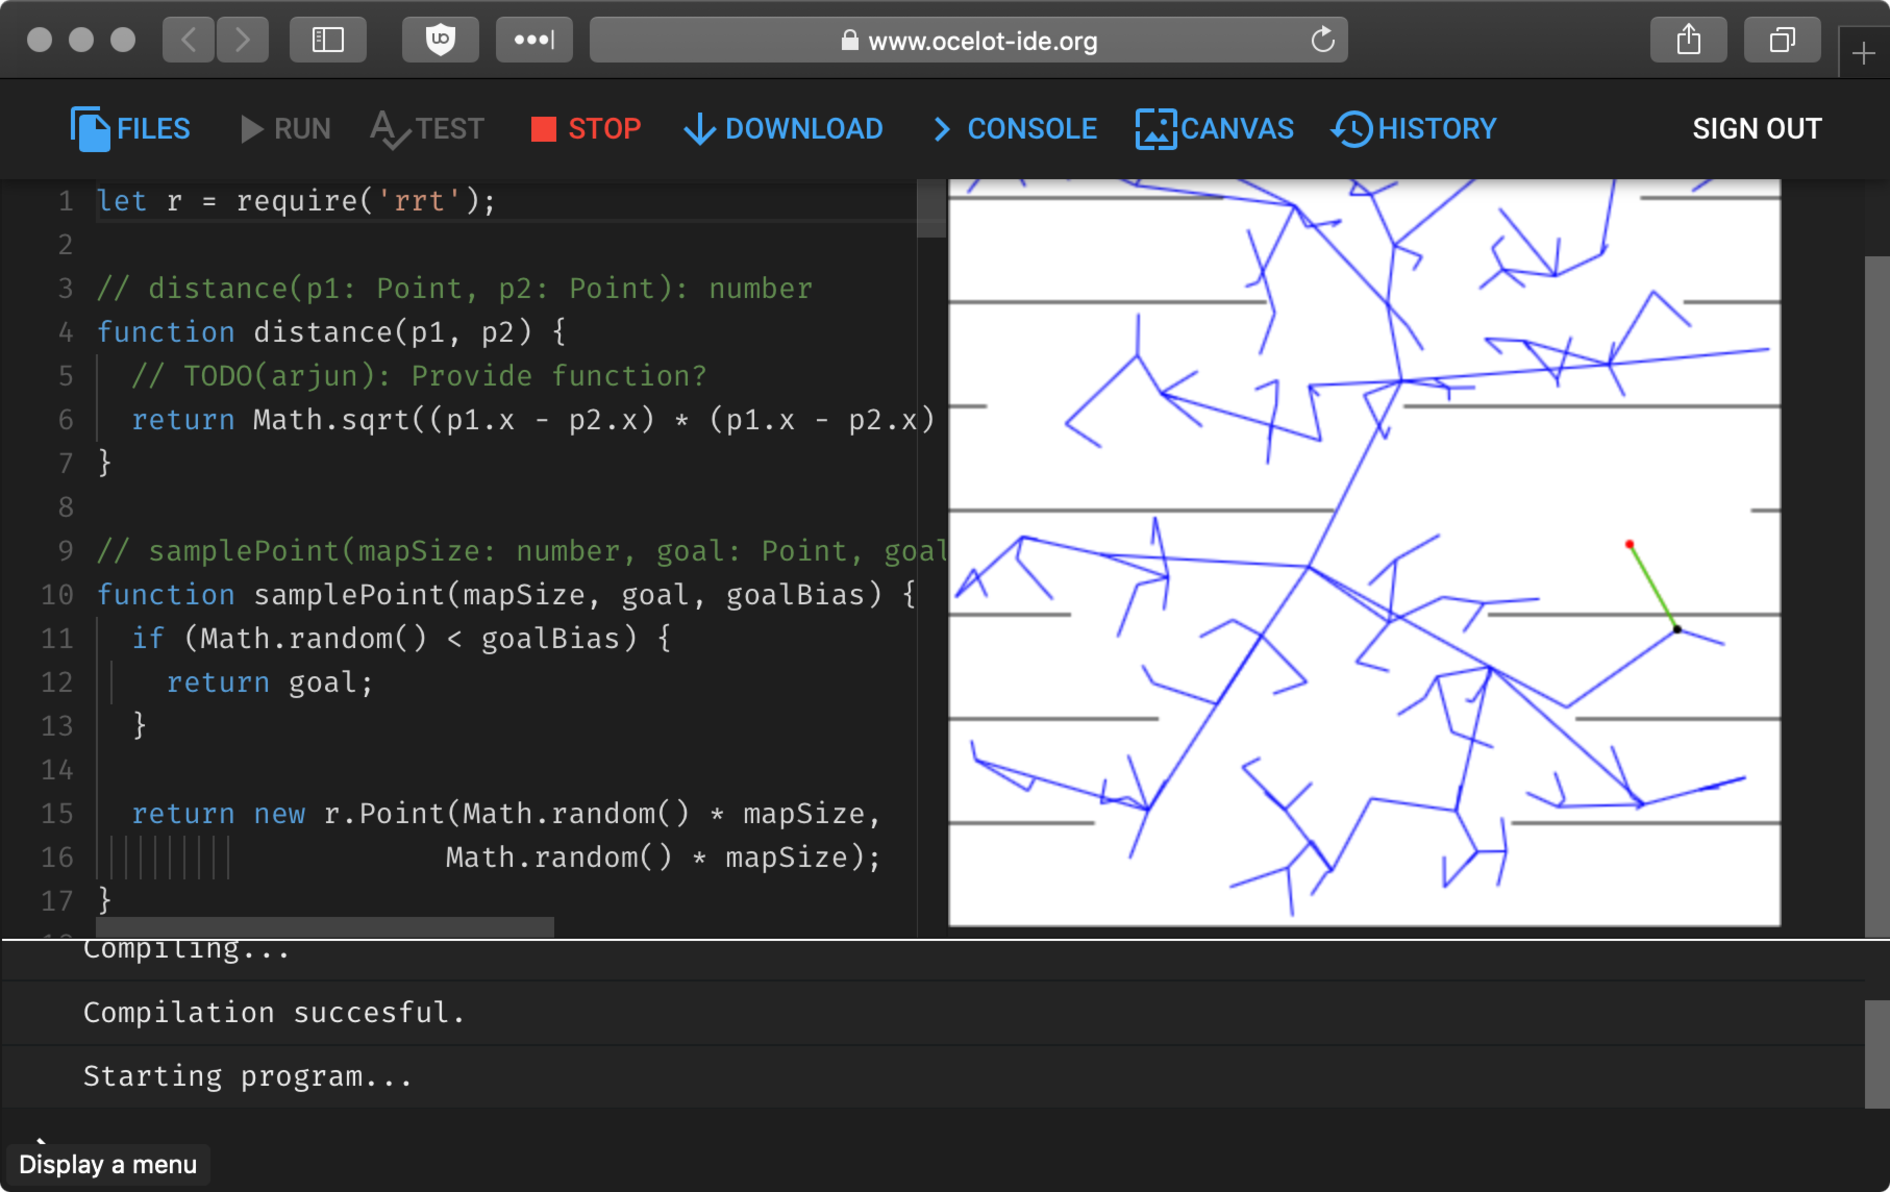
\includegraphics[width=0.9\textwidth]{ocelot_screenshot.pdf}
\end{center}

\begin{itemize}

    \item Used by 200-300 students each semester in a sophomore software engineering class

    \item Goal is \emph{not} to teach web programming

    \item Uses Stopify for synchronous I/O, long computations, stop button, etc.

\end{itemize}

\end{frame}

\begin{frame}[fragile]

\frametitle{Stopify Implementation: High-level idea}

\begin{itemize}

\item The Stopify compiler instruments each function to run in three
modes:

\begin{itemize}
    \item \emph{Normal mode:} function runs normally
    \item \emph{Capture mode:} function saves its own stack frame and
    returns to its caller, which does the same
    \item \emph{Restore mode:} function restores its local
    variables and jumps to the last statement it was executing
\end{itemize}

\item The Stopify runtime system manages the transitions between each mode

\item The \lstinline|control| operator sets the mode to capture

\item Applying a continuation value clears the stack and sets the mode to restore

\end{itemize}

\end{frame}

\begin{frame}[fragile]

\frametitle{Example}

\begin{columns}

\begin{column}{0.40\textwidth}
\begin{lstlisting}
var saved = "nothing yet";

function save(k) {
  saved = k;
}

function G(y) {
  console.log("Enter G");
  var z = control(save);
  return y + z;
}

function F(x) {
  console.log("Enter F");
  var s = G(x + 10);
  console.log(s);
}

F(0);
\end{lstlisting}

\end{column}

\begin{column}{0.55\textwidth}

\begin{itemize}
    \item How should we represent the continuation value captured
    at line 9?
    \item The continuation value must reconstruct the calls to \lstinline|F|
    and \lstinline|G|, without re-printing the output.
\end{itemize}

\end{column}

\end{columns}

\end{frame}

\begin{frame}[fragile]

\frametitle{Continuation Representation}

\begin{columns}

\begin{column}{0.4\textwidth}
\begin{lstlisting}
let saved = "nothing yet";

function save(k) {
  saved = k;
}

function G(y) {
  L1: console.log("Enter G");
  L2: var z = control(save);
  L3: return y + z;
}

function F(x) {
  L4: console.log("Enter F");
  L5: var s = G(x + 10);
  L6: console.log(s);
}

F(0);
\end{lstlisting}

\end{column}

\begin{column}{0.55\textwidth}

\begin{lstlisting}
let saved = [
    { f: F, l: L5, vars: { x: 0 } },
    { f: G, l: L2, vars: { y: 10 } }
];
\end{lstlisting}

\begin{itemize}

    \item In capture mode, each function pushes its own frame into the array

    \item In restore mode, each function stores its own stack frame and then
    applies the next function in \lstinline|kValue|

\end{itemize}

\end{column}

\end{columns}

\end{frame}

\begin{frame}[fragile]
\frametitle{Restoring Continuations}

\begin{alertblock}{}
Let's pretend we have the \lstinline|goto| control operator in JavaScript:
\end{alertblock}

\begin{columns}

\begin{column}{0.40\textwidth}

\begin{lstlisting}
function G(y) {
  if (mode === 'restore') {
    y = cont[0].vars.y;
    var l = cont[0].l;
    cont.shift();
    goto l;
  }
  L1: console.log("Enter G");
  L2: let z = control(save);
  L3: return y + z;
}

function F(x) {
  if (mode === 'restore') {
    x = cont[0].vars.x;
    var l = cont[0].l;
    cont.shift();
    goto l;
  }
  L4: console.log("Enter F");
  L5: let s = G(x + 10);
  L6: console.log(s);
}

F(0);
\end{lstlisting}

\end{column}

\begin{column}{0.55\textwidth}

\begin{lstlisting}
let saved = [
    { f: F, l: L5, vars: { x: 0 } },
    { f: G, l: L2, vars: { y: 10 } }
];
\end{lstlisting}

\begin{itemize}

    \item \lstinline|isRestoring| and \lstinline|cont| are variables set by
    the Stopify runtime system

    \pause

    \item The \lstinline|control| operator is implemented
    as a function
\end{itemize}

\begin{lstlisting}
function control(receiver) {
    if (mode === 'restore') {
        mode = 'normal';
        return /* continuation arg */;
    }
    else if (mode === 'normal') {
       // Start capturing
    }
    else {
        // impossible case
    }
}
\end{lstlisting}

\end{column}
\end{columns}

\end{frame}

\begin{frame}[fragile]
\frametitle{Capturing Continuations}

\begin{itemize}

\item To capture a continuation, the program has to
save its stack

\item The \lstinline|control| operator throws an exception
that contains an array

\item Each function will catch the exception and and
itself to the array

\end{itemize}

\pause

\begin{columns}

\begin{column}{0.42\textwidth}

\begin{lstlisting}[basicstyle={\fontsize{6.5}{6.8}\ttfamily}]
function G(y) {
  if (mode === 'restore') {
    ...
  }
  L1: console.log("Enter G");
  try {
    L2: var z = control(save);
  }
  catch (exn) {
    exn.stack.push({
      f: G, l: L2,
      vars: { y: y }
    });
    throw exn;
  }
  L3: return y + z;
}

function F(x) {
    if (mode === 'restore') {
      ...
    }
    L4: console.log("Enter F");
    try {
      L5: var s = G(x + 10);
    }
    catch (exn) {
      exn.stack.push({
        f: F, l: L5,
        vars: { x: x }});
      throw exn;
    }
    L6: console.log(s);
}

F(0);
\end{lstlisting}

\end{column}

\begin{column}{0.54\textwidth}

\begin{lstlisting}
let saved = [
    { f: F, l: L5, vars: { x: 0 } },
    { f: G, l: L2, vars: { y: 10 } }
];
\end{lstlisting}

\begin{lstlisting}
function control(receiver) {
    if (mode === 'restore') {
        ...
    }
    else if (mode === 'normal') {
        throw {
          stack: [],
          receiver: receiver
        };
    }
    else {
        // impossible case
    }
}
\end{lstlisting}

\end{column}
\end{columns}
\end{frame}

\begin{frame}[fragile]
\frametitle{Capture/Restore with Arbitrary Expressions}

\begin{columns}
\begin{column}{0.4\textwidth}

\begin{lstlisting}
function P(f, g, x) {
  return f(g(x));
}
\end{lstlisting}

Same approach:
\begin{lstlisting}

function P(f, g, x) {
  if (mode === 'restore') {
    ...
  }
  try {
    L1: return(f(g(x)));
  }
  catch (exn) {
    exn.stack.push(...);
    throw exn;
  }
}
\end{lstlisting}

\pause

Two serious issues:

\begin{itemize}
  \item During capture: we cannot (easily) determine if the exception was thrown
  by \lstinline|f| or \lstinline|g|.
  \item During restore: \lstinline|goto L1| always applies \lstinline|g| first,
  and there is no way to skip it and apply \lstinline|f|
\end{itemize}

\end{column}

\begin{column}{0.58\textwidth}
\pause

(Automatically) rewrite \lstinline|P| to the following equivalent
function:

\begin{lstlisting}
function P(f,g,x) {
  let t = g(x);
  return f(t);
}
\end{lstlisting}

\pause

\begin{alertblock}{A Normal Form}
Cormac Flanagan, Amr Sabry, Bruce F. Duba, and Matthias Felleisen.
The Essence of Compiling with Continuations. PLDI 1993.
\end{alertblock}

My other experiences with ANF:
\begin{itemize}

  \item Type system design
  \item Program verification
  \item Program analysis
\end{itemize}

\end{column}
\end{columns}

\end{frame}

\begin{frame}[fragile]
\frametitle{After A Normalization}
\begin{columns}
\begin{column}{0.49\textwidth}

\lstinline|P| after A Normalization:

\begin{lstlisting}
function P(f,g,x) {
  let t = g(x);
  return f(t);
}
\end{lstlisting}

Correctly instrumented version of \lstinline|P|:

\begin{lstlisting}
function P(f, g, x) {
  if (mode === 'restore') {
    f = cont[0].vars.f;
    g = cont[0].vars.g;
    x = cont[0].vars.x;
    let l = cont[0].l;
    goto l;
  }
  L1: let t;
  try {
    L2: t = g(x);
  }
  catch (exn) {
    exn.stack.push({ f: P, l: L2,
      vars: { f: f, g: g, x: x } });
    throw exn;
  }
  L3: return f(t);
}
\end{lstlisting}
\end{column}

\begin{column}{0.47\textwidth}

\pause

\begin{itemize}

  \item Note that \lstinline|P| does not capture/restore the application
  \lstinline|f(t)|

  \item Therefore, when capture starts within \lstinline|f|, the next
   frame saved in \lstinline|cont| will be frame of the
  caller of \lstinline|P|

  \item During restore, the caller of \lstinline|P| will restore
  the \lstinline|f|-frame (skipping the \lstinline|P|-frame)

  \item This is safe, because the \lstinline|P|-frame is ``useless'':
  it is merely: \lstinline|return f(t)|

  \item This lets you fudge \emph{proper tail calls}

\end{itemize}

\end{column}
\end{columns}

\end{frame}

\begin{frame}
\frametitle{JavaScript A Normalization Pipeline}

Doing this correctly was half the work.

Multi-step process:
\begin{enumerate}

  \item Desugar a few JavaScript features (e.g., \lstinline|var x, y;|)
  \item Add \lstinline|{ }| around loop/if bodies
  \item Eliminate all loops except \lstinline|while| loops
  \item Eliminate \lstinline|continue|
  \item Eliminate \lstinline|switch|
  \item Eliminate short-circuiting boolean expressions (e.g., \lstinline|f() \|\| g()|)
  \item A Normalize

\end{enumerate}

\pause

Approach:
\begin{enumerate}
  \item Straightforward assumptions and guarantees between each step
  \item Some steps are not fundamental, but simplify later stages
  \item Guiding principle: grammar of ANF-JavaScript
  \item Only one optimization: do not A-normalize expressions without
  applications (e.g., \lstinline|x + 1|\footnote{More later})
  \item Reusable artifact
\end{enumerate}

\end{frame}

\begin{frame}[fragile]
\frametitle{Implementing Continuations by Source to Source Translation}

\begin{enumerate}
  \item A Normalize JavaScript (7+ steps)
  \item Box assignable variables that are captured by nested functions and
  may be captured in continuations

  Analogous problem in compilers:
\begin{lstlisting}
function F(x) {
  function g(y) {
    return x + y;
  }
  return g;
}
let addTen = F(10);
addTen(5); // is x on the stack?
\end{lstlisting}

  \item Allow \lstinline|goto| to function applications
  \item Add capture/restore code to each function
  \item One optimization: avoid capturing code when it is obvious that
  the called function will not capture its continuation ($\approx30\%$ performance
  improvement)

\end{enumerate}

\end{frame}

\begin{frame}
\frametitle{JavaScript}

\begin{center}
Everything discussed so far is JavaScript-neutral, and is applicable
to other languages.
\end{center}

\end{frame}

\begin{frame}[fragile]
\frametitle{Arity Mismatch Errors}

\begin{itemize}

\item The \emph{arity} of a function is the number of arguments in takes.

\item An \emph{arity mismatch error} occurs when a function receives the wrong
number of arguments. In statically typed languages (e.g., Java), arity mismatch
errors occur before the program is run. In dynamically typed languages,
arity mismatch errors occur while the program is running.

\item JavaScript does not have arity mismatch errors.

\begin{lstlisting}
function F(x) {
  console.log(x);
}

F(1, 2); // prints 1. The 2 is ignored.
F(); // prints undefined.
\end{lstlisting}

\item This is not a problem for continuations

\end{itemize}

\end{frame}

\begin{frame}[fragile]
\frametitle{The ``arguments'' Object}

All the arguments of a function are available in the
\lstinline|arguments| object.

\begin{lstlisting}
function F(x) {
  console.log(x);
  for (let i = 0; i < arguments.length; i++) {
    console.log(arguments[i]);
  }
}

F(1,2,3,4); // prints 1 1 2 3 4
\end{lstlisting}

\begin{alertblock}{Problem}
This is a problem: we may lose the extra arguments during capture.
\end{alertblock}

\end{frame}

\begin{frame}[fragile]
\frametitle{Implicit Method Calls}

\begin{block}{Trivia}
Give value for \lstinline|x|, such that \lstinline|"Hello " + x| is an infinite
loop.

\pause

Hint: The same idea holds in Java too.
\end{block}


\pause

\begin{lstlisting}
let x = {
  toString() {
    while (true) { }
  }
}
\end{lstlisting}

\begin{alertblock}{Problem}
\begin{lstlisting}
let x = {
  toString() {
      control(...)
  }
}
\end{lstlisting}
\end{alertblock}

\end{frame}

\begin{frame}[fragile]
\frametitle{Solutions and Performance}

\begin{itemize}

  \item Problem: functions with arity mismatches
  \item Solution: save and restore the \lstinline|arguments| object\footnote{This does not work in the general case.}
  \item Performance problem: \lstinline|arguments| object materialization
  \pause
  \item Problem: implicit method calls,
  \item Solution: make the implicit calls explicit
\begin{lstlisting}
let t1 = x.toString(); // and valueOf
let t2 = "Hello " + t1;
\end{lstlisting}
  \item Performance problem: lots of extra instrumentation
  \pause
  \item Problem: JavaScript supports getters and setters:
\begin{lstlisting}
let a = o.b; // may call the getter b
\end{lstlisting}
  \item Solution: make the implicit calls explicit
  \item Performance problem: lots of extra instrumentation

\end{itemize}

\end{frame}

\begin{frame}
\frametitle{Solution: Ignore Problems When Possible}

\begin{block}{}
A compiler that produces JavaScript emits code into a sub-language of JavaScript.
\end{block}

\begin{tabular}{|l|c|c|c|c|l|}
\hline
\textbf{Compiler} & \textbf{Impl} & \textbf{Args} & \textbf{Getters} & \textbf{Eval} & \textbf{(\#) Benchmarks} \\
\hline
PyJS           & \xmark        & \textbf{M} & \xmark     & \xmark     & (16) PyPy Benchmarks, Shootout \\
ScalaJS        & \lstinline|+| & \xmark     & \xmark     & \xmark     & (18) Shootout \\
scheme2js      & \xmark        & \textbf{V} & \xmark     & \xmark     & (13) Larceny \\
ClojureScript  & \lstinline|+| & \textbf{M} & \xmark     & \xmark     & (8) Shootout \\
dart2js        & \lstinline|+| & \xmark     & \textbf{T} & \textbf{T} & (15) Ton80, Shootout \\
Emscripten     & \xmark        & \textbf{V} & \xmark     & \xmark     & (13) JetStream, Shootout \\
BuckleScript   & \xmark        & \xmark     & \xmark     & \xmark     & (15) OPerf-Micro, Shootout \\
JSweet         & \lstinline|+| & \textbf{M} & \xmark     & \xmark     & (9) SciMark, Shootout \\
JavaScript     & \cmark        & \cmark     & \cmark     & \cmark     & (19) Kraken, Shootout \\
Pyret          & \xmark        & \xmark     & \xmark     & \textbf{T} & (21) Pyret \\
\hline
\end{tabular}

\begin{itemize}

\item A \cmark{} or \xmark{} indicates that a JavaScript feature is used in
full or completely unused. The other symbols indicate restricted variants of
the feature.

\item Identifying the right sub-language can improve performance dramatically

\end{itemize}

\end{frame}

\begin{frame}
\frametitle{Example: Performance of PyJS}

\begin{columns}

\begin{column}{0.45\textwidth}
\begin{tikzpicture}
\node{\pgfimage[width=.95\columnwidth]{pyjs_case_study_sane_vs_insane.pdf}};
\end{tikzpicture}

\end{column}
\begin{column}{0.45\textwidth}
\begin{tikzpicture}
\node{\pgfimage[width=.95\columnwidth]{pyjs_case_study_new_method.pdf}};
\end{tikzpicture}

\end{column}

\end{columns}

Performance relative to unmodified PyJS on a suite of 10 Python benchmarks run
10 times each. Each graph shows how an option setting affects running time or
latency. Error bars show the 95\% confidence interval.

Speedups are a fluke, due to PyJS generating really bad code.

\end{frame}

\begin{frame}
\frametitle{Performance Evaluation}

\begin{center}
\begin{tikzpicture}
\node{\pgfimage[width=.87\textwidth]{all_slowdowns.pdf}};
\end{tikzpicture}
\end{center}

CDFs of Stopify's slowdown on nine languages. The median slowdown is in the
legend.

\end{frame}

\begin{frame}
\frametitle{PyJS + Stopify vs. Skulpt}

\begin{itemize}
  \item Skulpt: implementation of Python in JavaScript that does execution
  control
  \item PyJS: implementation of Python in JavaScript without execution
  control
  \pause
  \item Issues: (1) Skuplt can only run 8 of 16 benchmarks, (2) PyJS and Skulpt
  pass/fail different portions of the CPython test suite, (3) probably other
  threats to validity
\end{itemize}

\pause

\begin{center}
\begin{tabular}{|l|r|r|}
\hline
Benchmark & $\mu$ & 95\% CI \\
\hline
anagram & 0.25 & $\pm$ 0.01 \\
binary-trees & 0.27 & $\pm$ 0.01 \\
fib & 0.25 & $\pm$ 0.00 \\
gcbench & 0.08 & $\pm$ 0.01 \\
nbody & 0.25 & $\pm$ 0.00 \\
pystone & 0.37 & $\pm$ 0.01 \\
schulze & 1.25 & $\pm$ 0.08 \\
spectral-norm & 0.36 & $\pm$ 0.01 \\
\hline
\end{tabular}

Slowdown relative to Skulpt. (Stopify is faster when $\mu < 1$.)

\end{center}

\end{frame}

\begin{frame}[fragile]
\frametitle{Stopify + Pyret}

\begin{itemize}

  \item Joe Politz, one of Pyret's lead developers, co-authored this work

  \item Pyret: mostly-functional programming language that compiles to JS,
  self-hosting compiler, does proper tail calls, blocking I/O, REPL,
  animations, graceful termination, etc.

  \item Five years of engineering, thousands of users, still has some issues

  \pause
  \item Our approach: modify the last phase of the Pyret compiler and portions
  of the runtime system to invoke Stopify, instead of doing capture/restore
  itself (lots of code deleted)\footnote{This is the right way to use Stopify.}

\end{itemize}

\pause

From Pyret's runtime system (several bug fixes over the years):

\begin{lstlisting}[basicstyle={\fontsize{6}{6.2}\ttfamily}]
function eachLoop(fun, start, stop) {
  var i = start;
  function restart(_) {
    var res = thisRuntime.nothing;
    if (--thisRuntime.GAS <= 0) { res = thisRuntime.makeCont(); }
    while(!thisRuntime.isContinuation(res)) {
      if (--thisRuntime.RUNGAS <= 0) { res = thisRuntime.makeCont(); }
      else {
        if(i >= stop) {
          ++thisRuntime.GAS;
          return thisRuntime.nothing;
        } else {
          res = fun.app(i);
          i = i + 1;
    } } }
    res.stack[thisRuntime.EXN_STACKHEIGHT++] =
      thisRuntime.makeActivationRecord("eachLoop", restart, true, [], []);
    return res;
  }
  return restart();
}
\end{lstlisting}
\end{frame}

\begin{frame}[fragile]
\frametitle{Stopify + Pyret}

After Stopify (which generates equivalent instrumentation):

\begin{lstlisting}
function eachLoop(fun, start, stop) {
  for (var i = start; i < stop; i++) { fun.app(i); }
  return thisRuntime.nothing;
}
\end{lstlisting}

\begin{center}
\begin{tikzpicture}[baseline=0em]
\node{\pgfimage[width=0.75\columnwidth]{pyret_slowdown.pdf}};
\end{tikzpicture}
\end{center}

\end{frame}

\begin{frame}
\frametitle{Conclusions}

\begin{itemize}

  \item Use existing infrastructure when possible (in this case, Babel)
  \item When working on a full-scale language, identify a small fragment
  in which the essence of the problem and solution can be formulated
  \item The translation may be problem-dependent (e.g., type-checking
  vs translation)
  \item ANF is likely to help you
  \item Take testing and CI seriously

\end{itemize}

\end{frame}

\end{document}
